\documentclass[../main]{subfiles}
\ifSubfilesClassLoaded{
    \dominitoc
    \tableofcontentsfile
	\pagenumbering{arabic}
    \setcounter{page}{1}
}{}

\begin{document}
\graphicspath{{06-Analyse/figures},{../06-Analyse/figures}, {../06b-Analyse-2D}}

\chapter{Extension aux cartes en deux dimensions}

\minitoc
Nous avons étudié des comportements de base de cartes 1D sur des données en une dimension. Cependant, il est avantageux d'utiliser des cartes en deux dimensions sur des tâches de quantification vectorielle. 
Afin de généraliser le modèle à des données en dimension supérieures, nous avons cherché à observer ses propriétés d'auto-organisation, d'apprentissage et de prédiction sur des cartes en deux dimensions apprenant sur des données géométriques en deux dimensions.


\section{Entrées}

Nous travaillons à présent sur des entrées en deux dimensions. Pour analyser un cas géométrique similaire au cas en une dimension, les entrées sont des points en 4 dimensions pour une structure de 2 cartes, 6 dimensions pour 3 cartes. Ces points sont situés sur une sphère 3D dont on a effectuée une rotation dans l'espace de plus haute dimension, de la même façon que les entrées en 3D se trouvaient sur un cercle 2D dont on a effectué une rotation dans l'espace, voir figure~\ref{fig:sphere_inputs}. La variable $U$ paramétrant cette surface est en deux dimensions.
Comme pour les entrées prises sur une courbe, nous normalisons les entrées entre 0 et 1 sur chaque dimension, entrainant une légère déformation de la courbe.
Nous prenons une architecture de deux cartes, prenant chacune une paire de dimensions du point en 4D (respectivement 6D).

Nous comparerons les résultats obtenus sur cette disposition d'entrées à ceux obtenus sur des entrées indépendantes prises dans $[0,1]^4$. 

\begin{figure}
	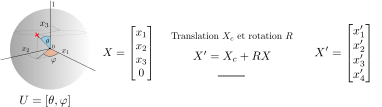
\includegraphics[width=\textwidth]{sphere_inputs.pdf}
	\caption{Transformation d'une surface d'un espace 3D en surface dans un espace 4D ou 6D. Les points restent positionnés sur une surface, mais sont plongés dans un espace de plus grande dimension. La rotation permet de répartir les coordonnées des points sur les dimensions. \label{fig:sphere_inputs}}
\end{figure}

\section{Organisation des poids}

Dans ces deux expériences, nous prenons des cartes 2D de taille $100x100$ prenant chacune des entrées 2D. Chacune des cartes est connectée à l'autre. Chaque carte a donc une couche de poids $\w\ext$ en deux dimensions, se dépliant sur les entrées externes, et une couche de poids contextuels $\w_c$, apprenant dans l'espace des positions de l'autre carte, donc en deux dimensions. Toutes les entrées sont normalisées.

Une première difficulté apportée par les deux dimensions est que l'organisation des poids externes n'est pas forcément assurée pour un rayon de voisinage constant, même dans une carte sans connexions contextuelles. Par exemple, l'organisation attendue d'une carte sur le carré $[0,1]^2$ est que les coins de la carte viennent dans les coins du carré. Cependant, les mécanismes d'organisation peuvent conduire à une carte tordue en son milieu.
% figure ??
Dans une architecture CxSOM, cela peut poser un problème pour l'utilisation de la position du BMU en tant que représentation de l'entrée~: la position du BMU n'est plus directement représentative de l'entrée. Deux entrées proches peuvent avoir leur BMU de chaque côté de la carte.
Nous n'avons pas exploré en pratique ces cas de figure qui peuvent être une limitation du modèle~; dans un premier temps, nous avons choisi de déplier les poids externes sur quelques centaines d'itérations préalablement aux poids contextuels, en prenant un grand rayon de voisinage $r_e = 0.5$. Ce grand rayon permet d'éviter les zones de torsion dans la carte. Après cette étape préalable, nous réduisons le rayon externe $r_e = 0.2$ et effectuons l'apprentissage des poids externes et contextuels comme décrit dans le modèle CxSOM. Les poids externes affinent alors leur apprentissage et les poids contextuels s'organisent sur une carte "bien dépliée".

\subsection{Organisation de cartes sur des entrées indépendantes}

Comme les entrées externes sont en deux dimensions, nous pouvons tracer la disposition de la grille dans l'espace des entrées.
Cette représentation est tracée en figure~\ref{fig:2som_cub_we}~; chaque point $p$ de la carte est positionné en $\w_e(p)$. Nous préférons utiliser une représentation à l'aide d'une carte de coloration pour les poids contextuels en figure~\ref{fig:2som_cub_wc}. Le pixel situé à la position $p$ sur l'image prend la couleur correspondant à la valeur de son poids contextuel $w_c$, définie par la carte de coloration tracée sur la figure.
Cette représentation est similaire à celle utilisée en une dimension et permet de faire apparaître clairement des motifs dans la disposition des poids.


Tracer les poids nous permet ici de comparer l'organisation d'une carte à celle observée en une dimension. Nous soulignons cependant que cette représentation ne permet pas de détecter quelles unités sont effectivement BMU lors d'un test.

Les poids contextuels ayant appris sur des entrées indépendantes font apparaître des motifs auto-organisés dans leur disposition. Les motifs sont similaires sur les deux cartes, traduisant un aspect systématique et non aléatoire. Nous avons également remarqué que la taille des motifs dépend de la valeur du rayon de voisinage contextuel.
Néanmoins, les poids restent centrés autour de $0.5$~: les points représentés en rouge sur la carte de coloration sont les valeurs effectivement prises par les poids contextuels des deux cartes. Pourtant, les positions des BMUs de chaque carte observées lors d'un test s'étendent bien sur toute la surface d'une carte.
Ce comportement rappelle le cas en une dimension. Des architectures de 4 cartes apprenant sur 4 entrées 1D indépendantes voient également leurs poids contextuels se moyenner. Ce comportement est à voir comme une limite des architectures de cartes, mais cette limitation est générale à des cartes une et deux dimensions.

\begin{figure}
\includegraphics[width=\textwidth]{sphere_rc005_evol_landscape}
\caption{Evolution des poids contextuels d'une architecture de deux cartes pour $r_c =0.05$. Les points sont représentés sous forme de carte de coloration à gauche et sous forme de disposition dans l'espace des positions sur la figure de droite. On observe une évolution régulière sous forme de motif en hélice, mais cette disposition évolue dans le temps. Après 700000 itérations, la figure semble se déformer vers de nouveaux motifs. Cette organisation ne converge pas.}
\end{figure}



\section{Organisation et prédiction sur des entrées dépendantes}

En figures~\ref{fig:2som_s_we} et \ref{fig:2som_s_wc}, nous effectuons les mêmes tracés que précédemment, sur des cartes ayant appris sur une sphère en trois dimensions plongée dans un espace en 4D et pivotée. $U$ est alors en deux dimensions.
Nous remarquons également la présence de motifs dans l'organisation des poids contextuels. Cette fois, les poids prennent bien des valeurs s'étendant sur toute la surface d'une carte.
Cependant, nous n'avons pas la certitude que cette disposition correspond à une position de convergence des poids. 
La taille des motifs dépend de la valeur de $r_c$. Nous comparons ainsi en figure~\ref{fig:2som_s_comp} les motifs obtenus sur une disposition de sphère, pour un rayon de voisinage correspondant à $r_c = 0.02$. Les motifs formés sont différents.



\begin{figure}
	\begin{minipage}{\textwidth}
		\centering\includegraphics[width=0.7\textwidth]{2SOM_CUB_we_199999.pdf}
		\label{fig:2som_cub_we}
	\end{minipage}
	\begin{minipage}{\textwidth}
		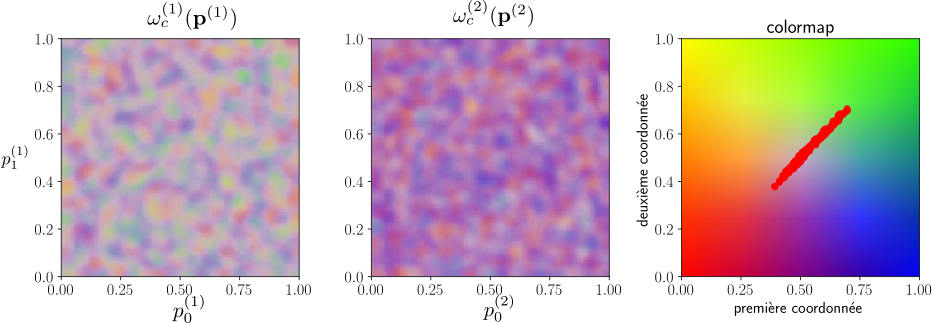
\includegraphics[width=\textwidth]{2SOM_CUB_wc_199999_v2.pdf}
		\caption{En haut: poids externes des cartes $M\m{1}$ et $M\m{2}$ représentés sous forme de distorsion de la carte après 200000 itérations.
	En bas: poids contextuels des cartes pour la même itération, représentés sous forme de carte de couleur en deux dimensions. Un pixel situé à la position $p_i,p_j$ prend comme couleur correspondante la valeur 2D de son poids contextuel, associé à une couleur par la carte de coloration représentée à droite de la figure.
	Les points rouges indiqués sur la carte de coloration sont les valeurs effectivement prises par toutes les valeurs de $\w_c^{(1)}$ et $\w_c^{(2)}$. On remarque donc que les poids contextuels ne se déplient pas sur toutes les valeurs prises par les BMUS.\label{fig:2som_cub_wc}}
	\end{minipage}
\end{figure}

\begin{figure}
	\begin{minipage}{\textwidth}
		\centering\includegraphics[width=0.7\textwidth]{2SOM_sphere_wc_249999.pdf}
		\label{fig:2som_s_we}
	\end{minipage}
	\begin{minipage}{\textwidth}
		\includegraphics[width=\textwidth]{2SOM_sphere_we_249999.pdf}
		\caption{En haut: poids externes des cartes $M\m{1}$ et $M\m{2}$ représentés sous forme de distortion de la carte après 200000 itérations.
		En bas: poids contextuels des cartes pour la même itération, représentés sous forme de carte de couleur en deux dimensions. Un pixel situé à la position $p_i,p_j$ prend comme couleur correspondante la valeur 2D de son poids contextuel, associé à une couleur par la carte de coloration représentée à droite de la figure.
		Les points rouges indiqués sur la carte de coloration sont les valeurs effectivement prises par toutes les valeurs de $\w_c^{(1)}$ et $\w_c^{(2)}$. On remarque donc que les poids contextuels ne se déplient pas sur toutes les valeurs prises effectivement par les BMUS.
		\label{fig:2som_s_wc}}
	\end{minipage}
\end{figure}


\begin{figure}
	\begin{minipage}{\textwidth}
		\centering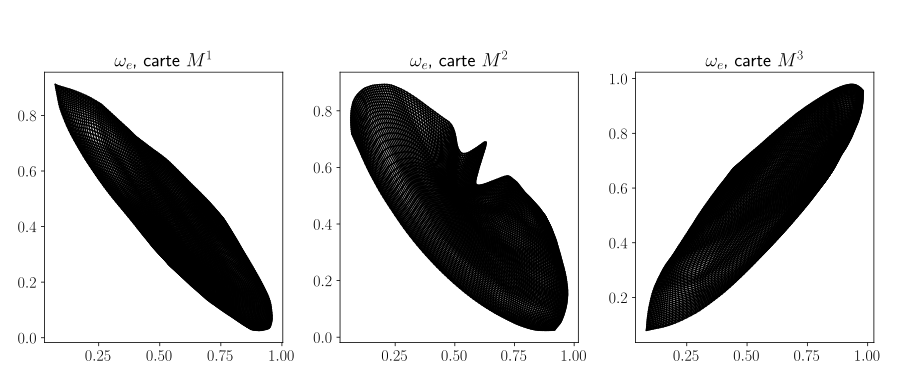
\includegraphics[width=0.7\textwidth]{3SOM_S_we_239999.pdf}
	\end{minipage}
	\begin{minipage}{\textwidth}
		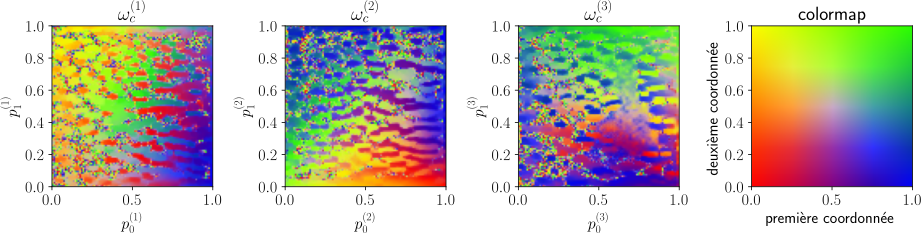
\includegraphics[width=\textwidth]{3SOM_S_wc_239999.pdf}
		\caption{}
	\end{minipage}
\end{figure}

\begin{figure}
\includegraphics[width=0.7\textwidth]{zclosed-1-239999_error.pdf}
\caption{Tracé de l'erreur de prédiction $\w_e\m{1}(X\m{1})$ en fonction de la valeur théorique de $X^{(1)}$, non présentée à l'architecture, dans une architecture de trois cartes 2D prenant des entrées $X^{(i)}$ en deux dimensions $[X^{(i)}_0, X^{(i)}_1]$. Nous traçons sur une ligne, pour chaque entrée, les dépendances entre chacune des dimensions.
Lorsque la carte $M^{(1)}$ ne reçoit pas d'entrée externe. Les cartes $M^{(2)}$ et $M^{(3)}$ ayant une activité externe, le graphique montre que la quantification vectorielle est bien réalisée dans ces cartes. La carte $M^{(1)}$ est uniquement activée par les connexions contextuelles venant de $M^{(2)}$ et $M^{(3)}$. La figure du haut montre que la prédiction est correctement réalisée.}
\end{figure}

\subsection{Limites}

La première limitation que nous observons avec des cartes en deux dimensions est une grande sensibilité aux conditions initiales selon les paramètres. 
Dans une première expérience, nous prenons $r_c = 0.02$ et $r_e = 0.2$.

Dans une seconde expérience, nous avons pris $r_c = 0.05$ et $r_e = 0.2$, sur les mêmes données d'entrées. 
Nous remarquons que l'expérience 2 conduit à une configuration stable des poids contextuels, dont certains ont convergé vers un point fixe et d'autres vers un cycle limite. 

L'expérience 1 présente des motifs instables qui évoluent au cours du temps. Nous remarquons une organisation des poids contextuels en hélice, qui 




%Convergence des cartes 2D Cottrell 


\ifSubfilesClassLoaded{
    \printbibliography
    %\externaldocument{../main.tex}   
}{}
\end{document}



% PLAN


% Convergence des poids :
% - Dépend des paramètres, contrairement à la carte en 1D on n'arrive pas forcément dans une position stable
% - Rc = 0.02 : point fixe, avec une partie 
% - Chaque expérience différente : grande dépendance aux conditions initiales. 